\chapter{Exploration of Alternative Systems}

There are three broad classes of material that have been explored as aero-engine blade material: metal alloys, ceramics and intermetallics.  Most metal alloys suitable for high-temperature application have been explored thoroughly over the last fifty years.  They suffer from decreases in strength at low homologous temperatures, have high densities and/or costs (W, Pt), and possess poor oxidation resistances (Mo, Nb, W).  Consequently, metal alloys have lower operating capabilities than intermetallics and ceramics, and are unsuitable for higher temperature operation.  

This leaves us with two categories of systems that have suitable candidates for high-temperature applications.  The first category are systems based on ceramics.  The options include: monolithic ceramics and ceramic matrix composites (CMCs).  The second category of systems are based on intermetallic phases.  The options are: monolithic or multi-phase intermetallics, metal-intermetallic materials. 

The academic community has identified various ceramic systems that have potential as successors to nickel-base superalloys.  Ceramics have very high melting points; some ceramics have the ability to retain strength at temperatures beyond 2000\celsius\ (Figure \ref{fig:CeramicsIntermetallics}).  However, the greatest hurdle faced by both monolithic ceramics and CMCs is their intrinsic lack of room temperature toughness ~\cite{evans80}.  Due to the nature of their atomic bonds, it is unlikely that this can be surmounted.  For this reason, we will not be exploring ceramics further in this work.

Several monolithic and multi-phase intermetallic systems are seen to offer a compromise between the room temperature robustness of superalloys and the high-temperature capabilities of ceramics ~\cite{nathal92, balsone01}.  Their room temperature toughnesses, however, are insufficient.  Several rather creative approaches that have been tried include:

\begin{enumerate}

\item ductile ligament toughening through utilising a softer second phase ~\cite{flinn89}
\item transformation toughening (which has been successfully employed in TRIP steels) ~\cite{evans86}
\item crack-deflection toughening ~\cite{strum94}
\item micro-crack toughening ~\cite{kumar91}
\end{enumerate}

Many stoichiometric intermetallics suitable for high-temperature applications do not have the fracture-toughness required for manufacture and processing ~\cite{kumar91}.  Intermetallic systems will hence not be considered in this work. 

Through this process of elimination, the thesis will focus on the options available in the realm of metal-intermetallic composites.
%
\begin{figure}[H]
\begin{center}
\includegraphics[width=\textwidth]{CeramicsIntermetallics}
\caption{Properties of ceramics and intermetallics compared to superalloys (adapted from ~\cite{nathal92}.) }\label{fig:CeramicsIntermetallics}
\end{center}
\end{figure}
%

Resistance to oxidation during exposure between room and operating temperatures is a neccessity for blade materials.  This prevents catastrophic failure through runaway oxidation occurring.  Whilst coatings may be used to protect the alloy, if the coating should fail in service, the alloy must possess sufficient oxidation resistance to survive between service intervals.  The three oxides through which oxygen has the lowest permeability are those of aluminium, chromium and silicon (Figure \ref{fig:oxidepermeability}).  To base our alloy system on one of these elements would be a sound start.

%
\begin{figure}[H]
\begin{center}
\includegraphics[width=11cm]{oxides}
\caption{The permeability of oxygen through various oxides vesus temperature ~\cite{nesbitt93}.}
\label{fig:oxidepermeability}
\end{center}
\end{figure}
%

\section{PGM Superalloys}

An extension of superalloy development based on platinum-group metals (PGMs) such as platinum, iridium and rhodium has been performed ~\cite{wenderoth05, mitarai98, mitarai97, mitarai99}.  These alloys are similar to nickel-base superalloys, and have a solid-solution matrix with a loading-bearing intermetallic L1$_2$ phase (Figures \ref{fig:ir17nb}).  The eutectic temperature between Ir solid-solution and Ir$_3$Nb is very high, at 2400\celsius\ (Figure \ref{fig:irnb}).  Casting this composition would be beyond the capabilities of most directional solidification (DS) facilities.  

The labyrinth structure of Ir-15at.\%Zr is similar to superalloys designed with very high misfit.  In Figure \ref{fig:LDSXInterrupted}, the microstructure of LDSX 8, a highly-misfitting superalloy, has many similarities to Ir-15at.\%Zr (Figure \ref{fig:ir17nb}b).  Such alloys have higher melting points than nickel-base superalloys and have the potential to operate at temperatures that are several hundred degrees higher than current superalloys ~\cite{okamoto94ir}.  

This alloy design approach has met with some success.  For instance, the 0.2\% flow stress of a binary PGM superalloy reached 1400  \mega\pascal\ at 1200\celsius\ (Figure \ref{fig:ir17nbi}) ~\cite{mitarai99}.  On the other hand, these alloys are three times denser than nickel-base superalloys and are also prohibitively expensive. 

 Although their densities make them unsuitable for moving parts, they may be well-suited for projects that operate on an essentially unlimited budget, such as inter-planetary rocketry missions.  It would be difficult to justify the costs that would be incurred for use in commercial jet engines.  We believe that there are better development options available, and will not be exploring PGM superalloys further in this work. 


%
\begin{figure}[H]
\begin{center}
\includegraphics[width=7.2cm]{ir17nb}
\includegraphics[width=6.75cm]{ir15zr}
\caption{(a) Microstructure of Ir-17Nb that has been heat treated at 1800\celsius\ for a day ~\cite{mitarai98}.  (b) Dark-field image of heat treated Ir-15at\% Zr, viewed from the [001] direction ~\cite{mitarai99}.}
\label{fig:ir17nb}
\end{center}
\end{figure}
%
%
\begin{figure}[H]
\begin{center}
\includegraphics[width=16cm]{irnb}
\caption{Binary phase-diagram of Ir and Nb ~\cite{okamoto94ir}.}
\label{fig:irnb}
\end{center}
\end{figure}
%
%
\begin{figure}[H]
\begin{center}
\includegraphics[width=16cm]{LDSXInterrupted}
\caption{Experimental nickel-based superalloys LDSX 1, 6 and 8.  They have increasing negative misfit from left to right.  These heat-treated specimens have been subject to tensile creep at 950\celsius/375 \mega\pascal.  The creep tests were stopped when the onset of secondary creep was observable.}
\label{fig:LDSXInterrupted}
\end{center}
\end{figure}
%
%
\begin{figure}[H]
\begin{center}
\includegraphics[width=8cm]{irflowstress}
\caption{0.2\% flow stresses of Ir alloys with -17at.\%Nb, -18Ta, -17Ti and -12Zr, when subject to compression tests at 1200\celsius\ ~\cite{mitarai99}.}
\label{fig:ir17nbi}
\end{center}
\end{figure}
%
\clearpage
\section{Alumina-Forming Alloys}

With the success enjoyed by nickel-based superalloys as high-temperature materials, there was a natural progression for research to concentrate on selected aluminides of nickel, titanium and iron in the 1980s and 1990s ~\cite{cotton93, miracle94a, walston93, white89, nathal92}.  

Ni$_3$Al and NiAl are the two nickel aluminides with melting-points higher than 1200\celsius\ (Figure \ref{fig:NiAl}) ~\cite{okamoto93}.  Ni$_3$Al is the intermetallic reinforcement phase in nickel-based superalloys.  It has a melting point of 1385\celsius, which is very close to the eutectic temperature of Ni--Ni$_3$Al.  In Figure \ref{fig:gpvolfrac}, an advanced single-crystal superalloy possessed the longest creep rupture life at 1000\celsius\ when it had a $\gamma$' volume fraction between 60-75\%.  This figure shows that the $\gamma$' volume fraction range for optimal creep performance of nickel-based superalloys is about 60--75\%  at temperatures between 780 and 1000\celsius.  A higher intermetallic content will not provide an increase in creep properties.  There is no benefit in designing an alloy without the toughening nickel solid-solution phase, as there would be no corresponding increase in high-temperature strength.

NiAl is a $\beta$2 phase with a melting point of 1638\celsius\ (Figure \ref{fig:NiAl}).  Its density of 5.92  \gram\usk\centi\rpcubic\meter\ is about 30\% lower than nickel-based superalloys ~\cite{okamoto93}.  The high-temperature properties of single-crystal and polycrystalline NiAl have been compared with Rene 80 in a Larson-Miller plot (Figure \ref{fig:NiAlLM}).  Rene 80 is a second generation nickel-based superalloy that is conventionally cast ~\cite{reed06}.  Single-crystal NiAl specimens outperform polycrystalline specimens at all temperatures tested, but both are vastly inferior to the third generation superalloy Rene80 (Figure \ref{fig:NiAlLM}). 

The anisotropic nature of DS-manufactured SX (single-crystal) NiAl can be seen in the differential in yield strength of NiAl grown in different orientations (Figure \ref{fig:NiAlys}) ~\cite{noebe96}.  The [100] orientation that shows superior strength at temperatures up to 400\celsius.  Above 400\celsius, [100] experiences a sharp reduction in yield strength.  The [110] orientation possess low yield strengths of 50--150MPa when above 100\celsius.  The [123] orientation has a slightly higher yield stress of 350-500 \mega\pascal\ above 200\celsius.  The orientation dependence of the yield stress arises because the normal slip systems are <100>\{010\}  and they cannot contribute to deformation along <100> because the resolved shear stress is zero on all such systems along <100>. Crystals stressed along <100> either kink, fracture or deform by operation of <111>\{110\} slip at low temperatures at very high stresses ~\cite{loretto71}.  The plastic deformation at these temperatures is associated with extensive dislocation climb because of the high concentration of thermal vacancies even at temperatures below 600\celsius\ ~\cite{fraser73a,fraser73b}.  These mid-to-high temperature properties are vastly inferior to superalloys.  The fracture-toughness of NiAl, like yield strength, is highest in the [100] direction ~\cite{kumar91}.

Alloying additions have improved mechanical properties at temperatures under 1000\celsius.  Co and Fe additions sit in the Ni-site of NiAl.  A Co content of about 40 at.\% increases NiAl creep resistance at 900\celsius\ most effectively across the Co and Fe contents tested (Figure \ref{fig:NiAlCo}) ~\cite{jung87}.  Other alloy additions such as Mo, the heusler phase and the TiB$_2$ phase have resulted in better high-temperature mechanical properties (Figure \ref{fig:NiAlLM}) ~\cite{miracle94a, walston93, darolia93, polvani76}, but due to the substantial softening at relative low temperatures of about 400\celsius, NiAl alloys have not been found to offer a mechanical advantage over superalloys at temperatures above 1100\celsius\ ~\cite{miracle94a}.
%
\begin{figure}[H]
\begin{center}
\includegraphics[width=14cm]{NiAl}
\caption{Binary phase-diagram of Ni and Al ~\cite{okamoto93}.}
\label{fig:NiAl}
\end{center}
\end{figure}
%
%
\begin{figure}[H]
\begin{center}
\includegraphics[width=10cm]{gpvolfrac}
\caption{Creep rupture life versus $\gamma$' volume fraction in an advanced single-crystal nickel-based superalloy, at 780\celsius/343MPa, and 68.6MPa, 98.0MPa and 117.6MPa at 1000\celsius\ ~\cite{harada82}.}
\label{fig:gpvolfrac}
\end{center}
\end{figure}
%

%
\begin{figure}[H]
\begin{center}
\includegraphics[width=15cm]{NiAlLM}
\caption{Rupture stress versus the Larson-Miller parameter for poly-crystalline and single-crystal NiAl, together with four other NiAl alloys.  Nickel-based superalloy Rene80 has been used as a bench-mark alloy ~\cite{walston93}.}
\label{fig:NiAlLM}
\end{center}
\end{figure}
%
%
\begin{figure}[H]
\begin{center}
\includegraphics[width=15cm]{NiAlys}
\caption{The yield stresses for the main orientations of NiAl between -200\celsius\ and 1000\celsius\ ~\cite{noebe96}.}
\label{fig:NiAlys}
\end{center}
\end{figure}
%
%
\begin{figure}[H]
\begin{center}
\includegraphics[width=12cm]{NiAlCo}
\caption{Creep resistances of (Ni,Fe)Al and (Ni,Co)Al at a creep-rate of 10$^{-7}$s$^{-1}$ at 900\celsius\ ~\cite{jung87}.}
\label{fig:NiAlCo}
\end{center}
\end{figure}
%

 
In Figure \ref{fig:LMplotforintermetallics}, the stress required for 1\% deformation versus log time has been plotted for various intermetallics and their constituent elements.  Single-crystal PWA 1480 has been used as bench-mark.  Nb$_2$Al (black square), the Nb aluminide with the higher Al content, is more creep resistant than Nb$_3$Al (upright white triangle) at 184MPa/1000\celsius.  The former would also have better resistance against `pesting' due to its higher Al content.

In Figure \ref{fig:darolia96}, the specific creep strength at a low temperature of 1027\celsius\ for SX, polycrystalline and eutectic (coupled with Ni solid-solution) NiAl have been plotted.  NiAl, when manufactured to give high strength, has inadequate fracture-toughness for aerofoil applications ~\cite{darolia96}.

The only high-temperature aluminide in the Co--Al binary is CoAl (Figure \ref{fig:coal}).  It has a melting point of 1640\celsius\ and a low density of 6.07 \gram\usk\centi\rpcubic\meter.  It is creep resistant at temperatures of 1000\celsius\ and below ~\cite{anton89, jung87}, and is unsuitable for higher temperature applications.  

%
\begin{figure}[H]
\begin{center}
\includegraphics[width=13cm]{darolia96}
\caption{Specific creep strength versus fracture-toughness for several classes of materials considered for high-temperature application ~\cite{darolia96}.}
\label{fig:darolia96}
\end{center}
\end{figure}
%

%
\begin{figure}[H]
\begin{center}
\includegraphics[width=14cm]{coal}
\caption{Binary phase-diagram of Co and Al~\cite{mcalister90}.}
\label{fig:coal}
\end{center}
\end{figure}
%


%
\begin{figure}[H]
\begin{center}
\includegraphics[width=10cm]{nbalys}
\caption{Yield strength of Niobium aluminides between room temperature and 1400\celsius.}
\label{fig:nbalys}
\end{center}
\end{figure}
%
Niobium aluminides have also been explored.  They show good high-temperature properties (Figure \ref{fig:nbalys}) up to about 1100\celsius.  Pure Nb$_3$Al has the highest yield strength at 1250\celsius, but it has poor oxidation resistance due to the formation of non-protective, volatile niobium pentoxide and AlNbO$_4$ during high-temperature exposure.  The Al content is not high enough to allow the alloy to form a protective alumina layer.  It is also susceptible to `pesting'.  Pesting is wide-scale, catastrophic, runaway oxidation of alloys at intermediate temperatures.  This occurs in many alloys containing Mo and Nb \cite{bewlay03, nesbitt93, ochiai06, shah92}.  Alloys that pest would experience uncontainable, uncontrollable, through-specimen oxidation in several hours.  Remnant alloy would not be found.  Pesting is many orders of magnitudes worse than the localised oxidation that has been seen in the latest generation nickel-based superalloys. Such localised oxidation would only extend 100\micro\metre\ from the original alloy surface; pesting, when it occurs, stops only when there is no alloy left that can be oxidised.


%
\begin{figure}[H]
\begin{center}
\includegraphics[width=5cm]{pest}
\caption{Pesting of a V--V$_3$Si alloy after 10 hours at 800\celsius.}
\label{fig:pest}
\end{center}
\end{figure}
%

Essentially, extensive efforts undertaken to improve the high-temperature mechanical properties of aluminides did not lead to increases in creep resistance.  They are believed to be unlikely to achieve higher temperature capabilities than nickel-base superalloys.


\section{Chromia-Forming Alloys}

Chromium oxide is known to be excellent for corrosion resistance; in fact, the principal method for making stainless steels stainless is through its addition.  Chromium oxide, however, has the unfortunate characteristic of volatilising at temperatures above 950\celsius\ ~\cite{perez02}, and is typically deemed unsuitable as the means of protection for operating temperatures that are to exceed 1100\celsius.  High-temperature alloys that form a chromium oxide layer would need another non-permeable oxide layer to sit atop it, such as a silica layer.


\section{Silica-Forming Alloys}

Silicon dioxide is stable up to 1650\celsius\ ~\cite{hallstedt92}, which is substantially higher than the target temperature capability of 1200\celsius.  Its adhesion to the underlying substrate, however, has not been extensively quantified.  Given the historical preference for alumina formers, it is suspected that silica may not be as adherent as alumina.  

Silicides have low to moderate densities, and exhibit excellent high-temperature oxidation resistances ~\cite{brady00}.  Several systems have been shown to demonstrate temperature capabilities that are almost 200\celsius\ higher than nickel-base superalloys ~\cite{schneibel03, sadananda99}.  For these reasons, attention has predominantly been focused on the development of refractory metal silicides.  However, there are significant deficiencies that must be overcome if these materials are to achieve widespread usage.  These include poor room temperature ductility, poor oxidation resistance at intermediate temperatures and in the presence of water vapour.  

As such, it remains uncertain whether these materials will ultimately be successful.  Additionally, the possibility that other parties, such as competing aeroengine manufacturers, are developing alternative materials based on systems other than those that have been published in the open literature cannot be dismissed.  An aim of this dissertation is to conduct an exploration of alloy systems containing silicide to identify those with the potential for high-temperature operation, have alloying capabilities with one another, and have the potential to exhibit damage tolerance at room temperature.


\section{Other Intermetallic Systems}

Strictly speaking, the constituents of pure intermetallics are metals; intermetallics should not contain semi-metallic elements such as Si.  Intermetallics composed of Cr, Nb, Co, Zr, Hf have been tested for their suitabilities as high-temperature materials.

The density-normalised stress for 1\% creep across 800--1500\celsius\ for intermetallics such as Fe$_2$Zr, Fe$_2$Nb and Cr$_2$Hf show that many of them posess poor mechanical properties at the minimum design requirement range of 800\celsius\ to 1200\celsius\ (Figure \ref{fig:conbzr}) ~\cite{anton92, kumar94hf}.  In the Larson-Miller plot comparing creep resistances of various intermetallics to SX PWA-1480 (Figure \ref{fig:LMplotforintermetallics}), Co$_2$Nb is less creep resistant than PWA-1480.  Cr$_2$Nb performs slightly better than the bench-mark superalloy.  Mo$_5$Si$_3$ (black upright triangle) out-performed all alloys tested.  Its excellent high-temperature mechanical properties has garnered Mo$_5$Si$_3$ much interest in the scientific community.  This will be detailed in Section \ref{subsection:MoSis}.

These intermetallics were found to be `extraordinarily hard' to fabricate into `crack-free' specimens due to their severely brittle nature ~\cite{anton92}.  Consequently, alloys designed with such phases must also contain a fracture-tough solid-solution phase, or the designed alloys would be rendered unmachinable.  A corresponding decrease in mechanical properties will accompany the inclusion of a solid-solution phase.

When designed well, some alloys are also not susceptible to pesting ~\cite{anton92, nesbitt93}; however, careful element selection is required for this to occur.
%
\begin{figure}[H]
\begin{center}
\includegraphics[width=12cm]{LMplotforintermetallics}
\caption{Larson-Miller plot of the stress for 1\% creep in steady state, comparing creep resistances of intermetallic compounds and their alloys against a single crystal superalloy, PWA 1480 ~\cite{anton89, anton89b, shah95}.}
\label{fig:LMplotforintermetallics}
\end{center}
\end{figure}
%
%
\begin{figure}[H]
\begin{center}
\includegraphics[width=10cm]{conbzr}
\includegraphics[width=10cm]{q}
\caption{(a) Density-normalised stress for 1\% creep in 300 hours for Co$_2$Zr, Co$_2$Nb, Fe$_2$Nb, Cr$_2$Nb and Nb$_2$Al, measured against several bench-mark poly-crystalline superalloys.  (b) Activation energy as a function of melting temperature for TCP intermetallics and relevant elements ~\cite{anton92}.}
\label{fig:conbzr}
\end{center}
\end{figure}
%


\section{Refractory Metal Silicide Systems}

In the last decade, the academic community has given molybdenum and niobium silicides the most attention.  Although they out-perform nickel-base superalloys in high-temperature creep, they form non-protective oxides at intermediate temperature ~\cite{ miracle94b, mitra06, ochiai06, sauthoff88, yanagihara96}.  Alloying can improve their oxidation resistance ~\cite{ramberg93, tomasi97, raj95a}, but can result in a decrease in high-temperature mechanical properties.

Low ambient temperature fracture-toughness is a common thread that runs through data on silicides explored for high-temperature applications  ~\cite{kumar94, miracle94b, shah92, sadananda99}.

Preliminary results show silicides with unoptimised microstructures containing micro-cracks display creep properties with a 200\celsius\ increase in temperature capability over nickel-base superalloys (Figures \ref{fig:creepshah92_1} and \ref{fig:creepshah92_2}).  However, these silicides have not been designed to contain a toughening phase and are very brittle, possessing poor fracture-toughness at room temperature.  Research thus far on molybdenum silicides and borosilicides, together with silicides of niobium, chromium, vanadium, titanium, tantalum and tungsten, will be described. 
%
\begin{figure}[H]
\begin{center}
\includegraphics[width=.75\textwidth]{creepshah92_1}
\vspace{-.3cm}
\caption{Measured elastic modulii of silicide systems and nickel-base superalloys between room temperature and 1200\celsius ~\cite{shah92}.}\label{fig:creepshah92_1}
\end{center}
\end{figure}
\vspace{-.5cm}
%
\begin{figure}[H]
\begin{center}
\includegraphics[width=.99\textwidth]{creepshah92_2}
\caption{Comparison of minimum compressive creep-rate of silicides and nickel superalloys vs stress between 1000--1400\celsius\ ~\cite{shah92}.}\label{fig:creepshah92_2}
\end{center}
\end{figure}
%



%
 			
\subsection{Molybdenum Silicides}\label{subsection:MoSis}

Molybdenum silicides have been heavily researched as they have high melting points of above 2000\celsius\ ~\cite{svechnikov70}, high-temperature strength-retention, and can possess good high-temperature oxidation resistance ~\cite{brady00, mitra06, raj95a,  ochiai06}.  However, they are susceptible to ``pesting" ~\cite{inui00, ochiai06, shah92, yanagihara96}.  This can be observed for MoSi$_2$ in the graph of mass change versus time in Figure \ref{fig:MoSi2_oxidation}.  At 500\celsius, MoSi$_2$ gains over 6\milli \gram\usk\centi\rpcubic\meter\ linearly.  In comparison, nickel-based superalloys gain substantially less than 1\milli \gram\usk\centi\rpcubic\meter\ in a parabolic fashion.  MoSi$_2$, despite being the molydenum silicide with the highest Si content, is unable to form a protective silica layer to prevent pesting.  Hot isostatic press (HIP) manufactured powder specimens fare better than cast specimens.  The smaller grains in HIP manufactured powder specimens allow for the short-circuit diffusion of Si through grain-boundaries to the oxidation zone.  This allows the specimens to form more protective silica-rich oxides; nonetheless, their oxidation rates are still linear.

There are three molybdenum silicides in the Mo--Si binary: Mo$_3$Si, Mo$_5$Si$_3$ and MoSi$_2$ (Figure: \ref{fig:MoSi}) ~\cite{svechnikov70}.  Molybdenum melts at 2620\celsius\ and has a density of 10.28  \gram\usk\centi\rpcubic\meter.  Mo$_3$Si has a density of 8.4  \gram\usk\centi\rpcubic\meter.  It undergoes a peritectic reaction at 2023\celsius.  This is very close to the eutectic temperature of MoSi$_3$ and Mo$_5$Si$_3$ at 2020\celsius.  Mo$_5$Si$_3$ melts at 2180\celsius, and has a lower density.  It forms a eutectic with MoSi$_2$ at 1900\celsius.  Molybdenum silicide alloys that do not contain molybdenum solid-solution can be slightly less dense nickel-based superalloys.  Alloys that contain Mo solid-solution tend to be heavier than superalloys; of course, this is dependent on phase fraction.
%
\vspace{6mm}
\begin{figure}[H]
\begin{center}
\includegraphics[width=11cm]{MoSi2_oxidation}
\caption{Mass change of MoSi$_2$ specimens, manufactured by either hot isostatic press (HIP) manufacture or casting, during oxidation at temperatures between 400--1400\celsius\ ~\cite{inui00}.}
\label{fig:MoSi2_oxidation}
\end{center}
\end{figure}
\vspace{-5mm}
%


%
\vspace{6mm}
\begin{figure}[H]
\begin{center}
\includegraphics[width=15cm]{MoSi}
\caption{The Mo-Si binary phase-diagram ~\cite{svechnikov70}}
\label{fig:MoSi}
\end{center}
\end{figure}
%

\clearpage
Mo$_3$Si is attractive as it can be in equlibrium with the ductilising solid-solution phase. The structural properties have been evaluated ~\cite{rosales00, swadener01}.  It has a low fracture-toughness of 3 \mega\pascal\m$^{\frac{1}{2}}$.  Its compressive strength at 1400\celsius\ was found to decrease with increasing Si content and decreasing strain-rate.  At 10$^{-3}$/s, Mo$_3$Si shows a yield strength of 660 \mega\pascal\ at a Si content of 22at.\%, and a yield strength of 300 \mega\pascal at a Si content of 25at.\%.   Mo$_3$Si has inferior yield strength to Mo$_5$Si$_3$.  Using atomic force microscopy, <100>\{010\} slip was observed in nano-indentation samples oriented in <100>, <110> or <111> orientations.  <100> was found to be the orientation with the highest indentation modulus ~\cite{swadener01}.

Mo$_5$Si$_3$ has been quite heavily researched because of its excellent high-temperature mechanical properties (Figure \ref{fig:LMplotforintermetallics}).  It has the highest melting point in the Mo--Si binary ~\cite{svechnikov70}.  The high-temperature structural performance of Mo$_5$Si$_3$ is related to its high-thermal stability and the existence of mixed metallic and covalent bonding within its crystal structure ~\cite{sakidja08}.  This structural performance is not confined only to the 5:3 molybdenum silicide; 5:3 silicides of Nb and Ti Mo$_5$Si$_3$ has poor room temperature fracture-toughness of 3  \mega\pascal\m$^{\frac{1}{2}}$\ and poor oxidation properties at intermediate and high-temperatures ~\cite{akinc99, anton89, anton89b}.  This is below the fracture-toughness threshold that would allow for specimen machining.  The inclusion of molybdenum solid-solution to provide a degree of plastic deformation decreases high-temperature performance, increases density and contributes to poorer oxidation behaviour.  

MoSi$_2$ has the best high-temperature oxidation resistance out of the molybdenum silicides due to its Si content.  Its susceptibility to pesting, as seen in Figure \ref{fig:MoSi2_oxidation}, can be mitigated by subjecting specimens to a pre-treatment at a high-temperature and low oxygen partial pressure to allow Si to form a protective silica layer.  No solution has yet been found for its poor fracture-toughness ~\cite{anton89, kishida10, shah95, shah92}.  Attempts at incorporating ductile solid-solution composing of W, Nb and Mo were met with failure ~\cite{dimiduk03}.  Interfacial interactions led to gross microstructural destabilisation.  Current consensus is that there is no feasible way to design MoSi$_2$-based alloys with sufficient creep, fracture and oxidation properties that would render them suitable for high-temperature structural applications ~\cite{dimiduk03, sekido07}.

Akinc has reported that 3 at.\% boron additions to Mo$_5$Si$_3$ improves its oxidation properties between 800 -- 1500\celsius\ by as much as 5 orders of magnitude (Figure \ref{fig:Mo5Si3_oxidation}).  During the initial onset of oxidation, a boro-silicate glass forms in competition with MoO$_3$.  MoO$_3$ is the cause of catastrophic oxidation of Mo$_5$Si$_3$; it sublimes at 750\celsius\ ~\cite{brewer90} and is non-protective.  The boro-silicate glass experiences viscous flow at 1000\celsius\ and promotes closure of sub-micron scale porosity left behind due to MoO$_3$ volatilisation; thus minimising subsequent oxidation of Mo into MoO$_3$ (Figure \ref{fig:MoSi_oxidationpictures}) ~\cite{akinc99}.  This is one reason why the scientific community believe that it is worthwhile to explore the Mo--Si--B system as an alloy design space for ultra-high-temperature applications. 


% 
\begin{figure}[H]
\begin{center}
\includegraphics[width=.95\textwidth]{Mo5Si3_oxidation}
\vspace{-.3cm}
\caption{Mass change of Mo$_5$Si$_3$ during oxidation at temperatures between 800--1500\celsius\ ~\cite{akinc99}.}\label{fig:Mo5Si3_oxidation}
\end{center}
\end{figure}
\vspace{-.5cm}
%
\begin{figure}[H]
\begin{center}
\includegraphics[width=.9\textwidth]{MoSi_oxidationpictures}
\vspace{-2mm}
\caption{SEM micrographs showing the transition of the initial oxide from MoO$_3$ to a boro-silicate glass ~\cite{akinc99}.}
\label{fig:MoSi_oxidationpictures}
\end{center}
\end{figure}
\vspace{-1cm}
%

\subsubsection{Molybdenum Borosilicide Alloys}

The Mo$_5$SiB$_2$ phase has been a focus of great interest to the high-temperature materials community due to its unparallelled creep properties at 1500\celsius\ ~\cite{hayashi04, ito01}.  This is a 400\celsius\ increase in creep capability over nickel superalloys.  At 1300\celsius, its creep-rate is about 3 orders of magnitude lower than a well-oriented MoSi$_2$ sample.  It is a boro-silicide variant of Mo$_5$Si$_3$.

The T$_2$ phase is a layered D8$_1$ crystal structure with a very high packing density (Figure \ref{fig:T2structure}) ~\cite{rawn01, sakidja08}.  The `A' and `A$_{\frac{1}{2}\frac{1}{2}}$' layers of pure Mo are sandwiched between layers of alternating Mo+Si and Mo+B layers.  At first glance, the layered structure could result in poor properties in shear, akin to that in graphite, but this has not been found to be the case.  The very large unit cell contains 20 Mo atoms, 4 Si atoms and 8 B atoms.  The large difference in atomic radii between Si and B ``neccessitates stacking arrangements" of the Mo layers such that distinct layers can be accommodated for Si and B.  

 
%
\vspace{8mm}
\begin{figure}[H]
\begin{center}
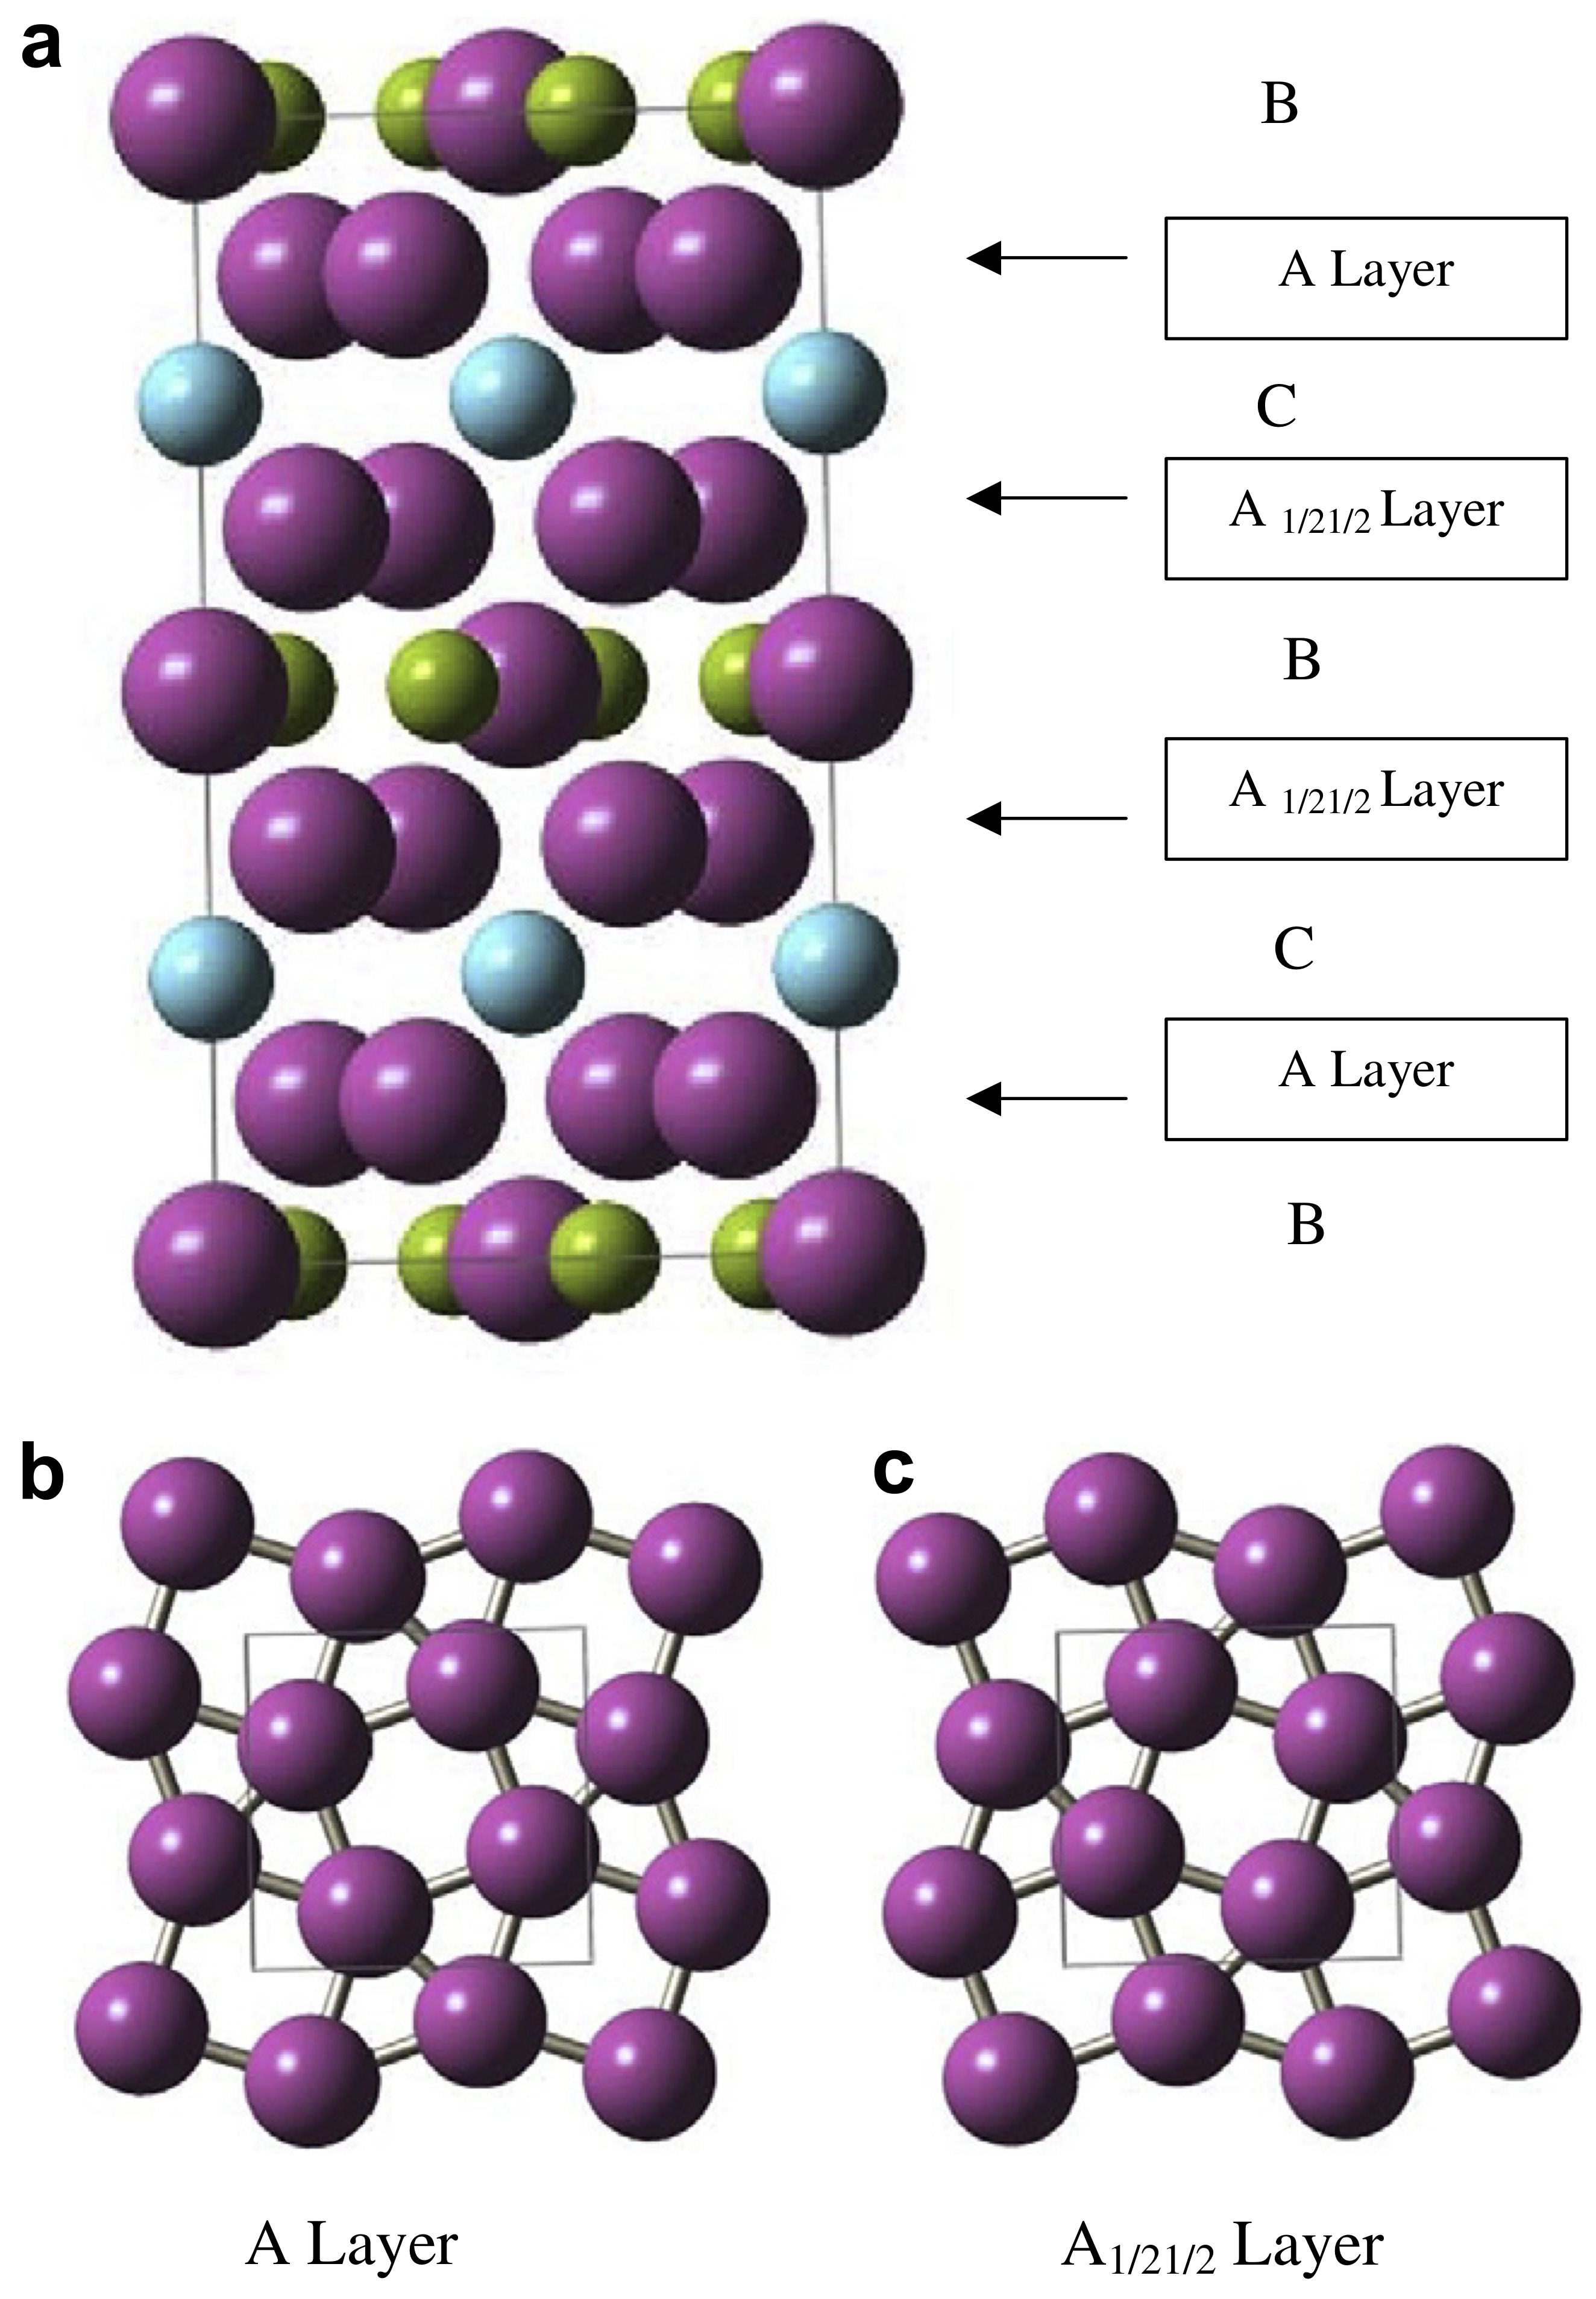
\includegraphics[width=9.5cm]{t2structure}
\caption{The crystal structure of Mo$_5$SiB$_2$ ~\cite{sakidja08}. }
\label{fig:T2structure}
\end{center}
\end{figure}
\vspace{-.2cm}
%
%
\begin{figure}[H]
\begin{center}
\includegraphics[width=\textwidth]{MoSiB_1600}
\caption{The ternary phase-diagram of Mo--Si--B ~\cite{nowotny57}.}
\label{fig:MoSiB_1600}
\end{center}
\end{figure}
%
%
\begin{figure}[H]
\begin{center}
\includegraphics[width=8.5cm]{Mo-Mo5SiB2}
\caption{Mo--Mo$_5$SiB$_2$ pseudo-binary phase-diagram ~\cite{yoshimi03}.}
\label{fig:Mo-Mo5SiB2}
\end{center}
\end{figure}
%
\clearpage
Nowotny et al. identified the T$_2$ phase in a 1600\celsius\ isothermal section of the ternary in 1957 (Figure \ref{fig:MoSiB_1600})  ~\cite{nowotny57}.  A Mo--Mo$_5$SiB$_2$ pseudo-binary phase-diagram has also been constructed by Yoshimi et al. (Figure \ref{fig:Mo-Mo5SiB2}) ~\cite{yoshimi03}.    An alloy of T$_2$ particles in a solid-solution matrix, when subject to compression-creep at different temperatures and strain-rates, show a range of deformation behaviour ~\cite{alur04}.  Brittle fracture, plastic deformation and elastic deformation were all observed.  

Perepezko has explored the influence of microstructure control in the manufacture of Mo--Mo$_5$SiB$_2$ and Mo--Mo$_3$Si--Mo$_5$SiB$_2$ for ultra-high-temperature applications (Figure \ref{fig:Mo16Si8B}) ~\cite{perepezko01}.  The ternary eutectic is difficult to attain via casting because solidification segregation causes very stable borides and silicides to form instead.  Also, the liquidus-surfaces for Mo$_3$Si and T$_2$ around the ternary eutectic region are shallow (Figure \ref{fig:MoSiB_liquidus}).  The invariant eutectic can be by-passed during non-equilibrium solidification.  Mo$_3$Si and T$_2$ would form instead, and there will be very little toughening component in the microstructure (Figures \ref{fig:Mo16Si8B} and \ref{fig:MoSiB_witheutectic}).

Perepezko has introduced alloying elements such as Nb to stabilise the T$_2$ phase and destabilise boride reactions (Figure \ref{fig:MoSiB_withNb}) ~\cite{perepezko01, sakidja00}.  Nb can substitute for Mo to a large extent in solid-solution and T$_2$.  This increases microstructural control and allows for direct solidification of a two-phase solid-solution and T$_2$ alloy in the region shaded in the liquidus-projection (Figure \ref{fig:Mo19Nb12Si8B}). 

%
\begin{figure}[H]
\begin{center}
\includegraphics[width=11cm]{Mo16Si8B}
\caption{SEM micrograph of arc-melted Mo--16.8Si--8.4B ~\cite{perepezko01}.}
\label{fig:Mo16Si8B}
\end{center}
\end{figure}
%
%
\begin{figure}[H]
\begin{center}
\includegraphics[width=14cm]{MoSiB_liquidus}
\vspace{-3mm}
\caption{The relevant portion of the Mo--Si--B liquidus projection T = 1873K ~\cite{perepezko01}.}\label{fig:MoSiB_liquidus}
\end{center}
\end{figure}
\vspace{-5mm} 	
%
%
\begin{figure}[H]
\begin{center}
\includegraphics[width=10cm]{MoSiB_witheutectic}
\caption{Microstructure of an alloy with T$_2$ as the primary phase with a Mo(ss)--T$_2$--Mo$_3$Si invariant ternary eutectic ~\cite{perepezko01}.}
\label{fig:MoSiB_witheutectic}
\end{center}
\end{figure}
\vspace{.7cm} 
%
\begin{figure}[H]
\begin{center}
\includegraphics[width=\textwidth]{MoSiB_withNb}
\caption{Increase in solid-solution volume-fraction in the ternary eutectic with Nb-alloying ~\cite{perepezko01}.}\label{fig:MoSiB_withNb}
\end{center}
\end{figure}
%
\begin{figure}[H]
\begin{center}
\includegraphics[width=9cm]{Mo19Nb12Si8B}
\caption{SEM micrograph of a polished section of cast and annealed Mo--19.5Nb--12Si--8.5B (at.\%) ~\cite{perepezko01}.}\label{fig:Mo19Nb12Si8B}
\end{center}
\end{figure} 
%

The dislocations formed in annealed alloys containing Mo$_5$SiB$_2$ are mostly of edge character with Burgers vectors of <100], 1/2<111], and <110], implying either that screw dislocations are far more mobile then edge dislocations and/or that the dislocations observed are formed from condensation of vacancies.  It has been suggested ~\cite{sekido07} that these vacancies are formed in Mo-rich alloys of Mo$_5$SiB$_2$.  The edge dislocations that form when these vacancies aggregate act as heterogeneous nucleation sites for subsequent Mo precipitation.  In Mo-lean Mo$_5$SiB$_2$, defects that form do not contribute to dislocation formation ~\cite{sekido07}.

%
\begin{figure}[H]
\begin{center}
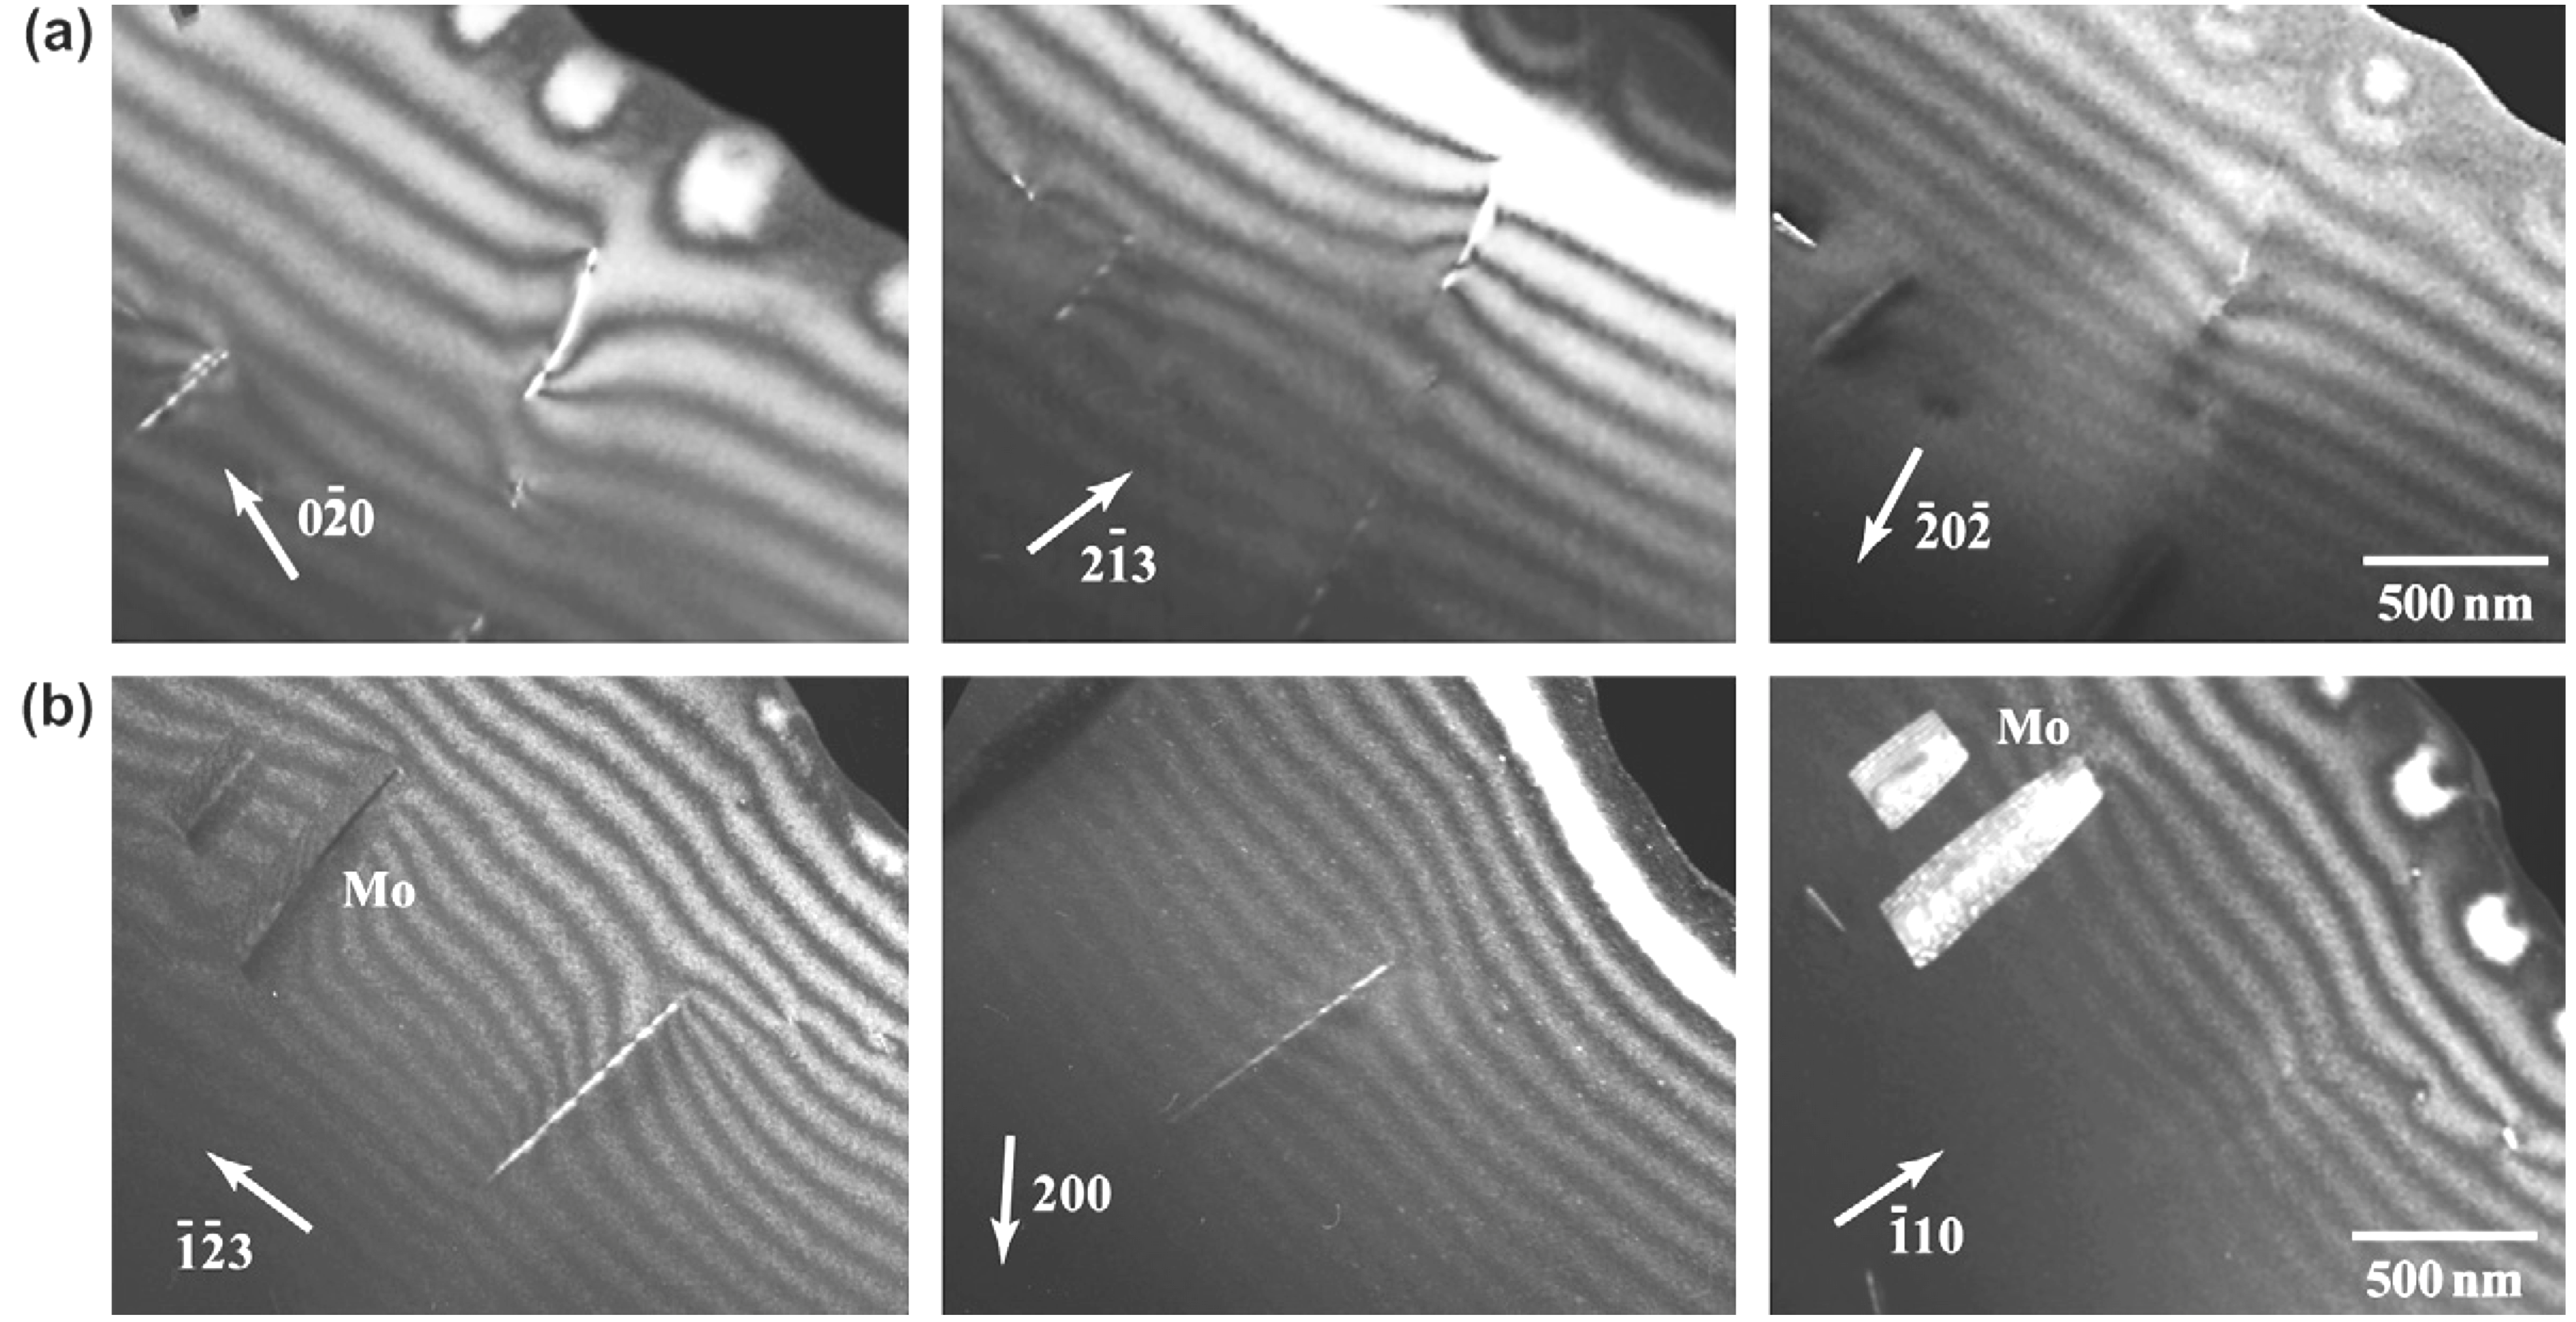
\includegraphics[width=16cm]{sekido07}
\caption{ Weak-beam dark-field images showing dislocations in Mo-rich T$_2$ phase.  The specimen was annealed for 20 hours at 1550\celsius.  The Burgers vector of the dislocations are (a) [010] and (b) [-1-10􏰇] ~\cite{sekido07}.}
\label{fig:sekido07}
\end{center}
\end{figure} 
%

A Mo--Si--B alloy was measured to have fracture-toughness values of 8 \mega\pascal\,m$^{\frac{1}{2}}$ at ambient temperature, to 25 \mega\pascal\,m$^{\frac{1}{2}}$ at 1400\celsius\ ~\cite{alur06}.  This is higher than the 3 \mega\pascal\,m$^{\frac{1}{2}}$ reported for molybdenum silicide alloys without a toughening solid-solution phase.  The dominant creep mechanisms in this alloy were found to be grain-boundary diffusion between 900--1200\celsius, and volume diffusion between 1200--1400\celsius.

In recent work ~\cite{kumar10}, the tensile creep properties of HIP-manfactured Mo--Si--B alloys have been successfully evaluated.  Tensile tests at a creep-rate of 10$^{-4}$s$^{-1}$ between 1000\celsius\ and 1200\celsius\ were performed on a solid-solution alloy, a solid-solution and ~35vol.\% T$_2$ alloy, and a solid-solution, T$_2$ and Mo$_3$Si alloy (Figure \ref{fig:ku10}).

%
\begin{figure}[H]
\begin{center}
\includegraphics[width=7.8cm]{ku10i}
\includegraphics[width=7.8cm]{ku10ii}
\vspace{5mm} 
\includegraphics[width=7.8cm]{ku10iii}
\caption{Tensile stress-strain curves from tests conducted at a nominal strain-rate of 10$^{-4}$ s$^{-1}$, at temperatures between 1000\celsius\ to 1200\celsius\ for (a) an Mo solid-solution alloy with <5vol.\% T$_2$ phase, (b) a two-phase alloy with solid-solution and T$_2$ phase (35 vol.\% ), (c) a three-phase alloy with solid-solution, T$_2$ and Mo$_3$Si ~\cite{kumar10}.}\label{fig:ku10}
\end{center}
\end{figure} 
%

In other recent work, this X$_5$SiB$_2$ phase has been described as a common 5:3 metal--metalloid compound that exists in many systems ~\cite{sakidja08}.  It is present in the Nb--Si--B ternary ~\cite{nunes97}, the V--Si--B ternary ~\cite{rodrigues09}, the Co--Si--B ternary, the Fe--Si--B ternary, the Mn--Si--B ternary, and the (Pt, Ir, Rh, Ru)--Si--B  ternaries ~\cite{sakidja08}.  Cr, Ta, W, Ti, Zr and Hf are all soluble to varying extents in this phase ~\cite{perepezko01, sakidja00, sakidja05, sakidja08}.  There is an ``unusually large"  refractory metal solubility in the Mo sites in the T$_2$ phase ~\cite{sakidja08}.

The mechanical and oxidation properties of T$_2$-containing alloys from the Mo--Si--B system are promising.  There are several viable alloying additions that stabilise the T$_2$ phase and the solid-solution phase.  Some alloying additions destabilise undesirable boride phases and the X$_3$Si phase.  These factors allow a degree of freedom in subsequent multi-phase alloy design.  Prototype protective oxidation bond coats for these alloys have also been developed ~\cite{perepezko10}.  Kinetics and reactive diffusion pathway analysis have been utilised in the design of a borosilicide coating that has a multi-layer phase-sequencing that allows for thermodynamic compatibility and an underlying diffusion barrier between the bond coat and the underlying substrate ~\cite{perepezko10}.  During high-temperature exposure, the bespoke coating has been elegantly designed to evolve in such a way such that its life is prolonged.

The evolution of Mo--Si--B alloys over the last two decades illustrates that substantial progress can be made when a judicious, strategic alloy design approach is coupled with appropriate, bespoke testing.  These alloys can be reasonably considered as bench-mark alloys for high-temperature structural materials.



\subsection{Niobium Silicides}

Nb--Nb$_3$Si alloys have been the focus of much research, partly because of their low densities and good high-temperature mechanical properties, ~\cite{jackson96, fleischer87, fleischer94, sauthoff88, shah92, bewlay03, miura09, balsone01}.  These characteristics allow for greater design flexibility.  Niobium silicides have poorer oxidation resistance than their molybdenum counterparts, pesting at low and intermediate temperatures ~\cite{ramberg93}.  They have poor room temperature fracture-toughness.  These issues have yet to be resolved ~\cite{jackson96, fleischer87, fleischer94, sauthoff88, shah92, ramberg93, bewlay03, mitra06}.

There are three niobium silicides in the Nb--Si binary: Nb$_3$Si, Nb$_5$Si$_3$ and NbSi$_2$ (Figure \ref{fig:NbSi}).  Niobium has a density of 8.57  \gram\usk\centi\rpcubic\meter, and Nb$_3$Si has a density of 7.52  \gram\usk\centi\rpcubic\meter.  The eutectic between niobium solid-solution and Nb$_3$Si has been looked at ~\cite{kimura05}, but there are many phase transitions between room temperature and the eutectic melting point (Figure \ref{fig:NbSi}).  At 1765\celsius, Nb$_3$Si undergoes a eutectoid decomposition to Nb and Nb$_5$Si$_3$.  To further complicate matters, Nb$_5$Si$_3$ has two allotropes.  The high-temperature phase is D8$_{m}$, and the low temperature phase is D8$_1$.  D8$_1$ has high strength at elevated temperatures ~\cite{bewlay01}.  The transformation temperature ranges between 1650\celsius\ and 1940\celsius\, and varies with composition.  This makes the manufacturing process for the D8$_1$ phase more complicated.  These transformation temperatures are well above the target operating temperature of 1200\celsius.  Once manufactured, the D8$_1$ phase should be stable.

%
\begin{figure}[H]
\begin{center}
\includegraphics[width=12cm]{NbSi}
\vspace{-2mm}
\caption{The Nb--Si binary phase-diagram ~\cite{okamoto90}.}\label{fig:NbSi}
\end{center}
\end{figure}  
%

In a two-phase alloy of Nb solid-solution and $\alpha$--Nb$_5$Si$_3$,  dislocations developed in the intermetallic when the alloy was compressed at 1673K.  Three types of slip systems operating are: \{011\}<111], \{001\}<100] and \{010\}<100] ~\cite{sekido10}.

Hypoeutectic alloys have dendrites of Nb solid-solution with an inter-dendritic eutectic consisting of a Nb$_3$Si matrix with fine Nb rods and ribbons aligned with the primary growth direction.  Hypereutectic alloys were found to contain primary Nb$_3$Si and Nb$_5$Si$_3$ dendrites with inter-dendritic eutectic.  The fracture-toughnesses of these materials ranged from 5.8  \mega\pascal\usk\meter$^{\frac{1}{2}}$ at the eutectic composition to 14.2  \mega\pascal\usk\meter$^{\frac{1}{2}}$ for a hypoeutectic composition at 10 at.\% Si, which are significantly better than monolithic Nb$_5$Si$_3$ ~\cite{strum94}.  In fact, the fracture-toughness for the latter is close to the minimum threshold for fracture-toughness of 15 \mega\pascal\usk\meter$^{\frac{1}{2}}$ ~\cite{shah95}.  However, the addition of the niobium matrix decreases creep strength by an order of magnitude at 1200\celsius, with minimum creep-rates comparable to those of nickel-base superalloys.  

Specimens used in high-temperature structural testing are mostly made using HIP manufacture of powder.  Ingots have been successfully made through conventional DS manufacturing, with the help of minor Sn or Ag additions ~\cite{bewlay03, vellios10}.

The extent of oxidation resistance in niobium silicide alloys positively correlates with Si content ~\cite{xiong09}.  Oxidation kinetics for Nb--10at.\%Si and Nb--20at.\%Si were similiar at 1000\celsius\ and 1200\celsius; specimens experienced linear oxide growth rates.  Mo, Ta and W have been used as alloying additions that would contribute to high-temperature strength.  Nb--20Si--10W had a parabolic oxide growth rate, and its weight increase was only about a quarter of the Nb--Si alloys.  WO$_3$ formed during thermal exposure, and although it is oxygen permeable, it is less volatile than MoO$_3$.  This ternary alloy showed higher oxidation resistance than  the quaternary alloy Nb--20Si--10W--10Mo.  Al, Cr and Ti additions to Nb--Nb$_5$Si$_3$ improved oxidation behaviour, but oxidation growth rates remained linear even after 100 hours of isothermal exposure at 800\celsius\ ~\cite{zelenitsas06}.  The alloy that had 5at.\%Cr formed a very thick oxide layer (Figuree \ref{fig:zelenitsas}).  The thinner oxide layer that formed on the alloy containing all three element additions spalled off upon cooling (Figure \ref{fig:zelenitsas}b).  It still had a significant thickness of several \milli\metre.

%
\begin{figure}[H]
\begin{center}
\includegraphics[width=4.5cm]{zelenitsas}
\includegraphics[width=5.3cm]{zelenitsasii}
\vspace{-2mm}
\caption{ Photographs of Nb--Nb$_5$Si$_3$ alloys containing (in at.\%) (a) 5Cr and (b) 24Ti--8Cr--4Al that had been subjected to 800\celsius\ for 100h ~\cite{zelenitsas06}.}\label{fig:zelenitsas}
\end{center}
\end{figure}  
%

To improve oxidation resistance in Nb alloys, Shah has attempted to attain a microstructure of Cr$_2$Nb and Si in a Nb--Cr--Si solid-solution matrix to increase Si content in the alloy ~\cite{shah95}.  Results were not encouraging; this is believed to have been caused by a complex intersection of liquidus surfaces.  Bewlay has added Ti, Al, Cr and Hf to improve oxidation properties ~\cite{bewlay03}.

Niobium is an alloying element that can positively contribute to other metal-silicide alloy systems.  It improves oxidation behaviour in Ti-Al and Zr-based alloys ~\cite{zhan09}.  The (Nb,Mo)s.s.--(Nb,Mo)$_5$Si$_3$ eutectic system shows good high-temperature mechanical properties.  However, the issue of poor oxidation resistance has not been adequately addressed in this system.  


\subsection{Chromium Silicides}
%
There are four chromium silicides in the Cr--Si binary: Cr$_3$Si, Cr$_5$Si$_3$, CrSi and CrSi$_2$ (Figure \ref{fig:CrSi}) ~\cite{gokhale90}.  We are interested in Cr$_3$Si as our strengthening phase because it is the intermetallic that can co-exist with the BCC chromium solid-solution phase.  There has been some research conducted on Cr$_5$Si$_3$, and like other intermetallics that have not been ductile-phase toughened, it has been shown to be brittle at room temperature.  All phases of this binary have low density.  The density of the solid-solution, the densest phase, is 6.91  \gram\usk\centi\rpcubic\meter.  The density of the Cr-rich intermetallic, Cr$_3$Si, is 6.47  \gram\usk\centi\rpcubic\meter.  Both densities are substantially lower than nickel-based superalloys.  Cr is BCC (Figure \ref{fig:BCC}) and Cr$_3$Si is A15 (Figure \ref{fig:A15}).  

%
\begin{figure}[H]
\begin{center}
\includegraphics[width=.9\textwidth]{CrSi}
\caption{The Cr--Si binary phase-diagram.}\label{fig:CrSi}
\end{center}
\end{figure}
%
%
\begin{figure}[H]
\begin{center}
\includegraphics[width=7cm]{BCC}
\caption{The body centered cubic structure of the solid-solution ~\cite{ashcroft76}.}\label{fig:BCC}
\end{center}
\end{figure} 
%
The low density constituent phases in this binary allow for alloys to be designed with substantial solid-solution content.  Alas, utilising Cr solid-solution as a toughening phase in alloys is a rather difficult matter.  Cr is known to suffer from nitrogen-embrittlement and notch-sensitivity at ambient temperature.  This makes Cr-based alloys crack-prone, and they are difficult to manufacture using conventional casting techniques.  They are also difficult to process and machine.  Extensive research into alloying elements to decrease the ductile-brittle transition-temperature (DBTT) did not achieve DBTTs below room temperature (Figure \ref{fig:Cr_ductility}) ~\cite{abrahamson57}. Most precious group metals (PGMs) were not tried as alloying additions because of their high costs.  Cr's DBTT can be most effectively brought down to 40\celsius\ by 4-6at.\% additions of Ru.  This DBTT is not ideal as it is above room temperature.  Such high Ru content would substantially increase alloy density, material costs and alloy density. This would decrease the attractiveness of Cr-based alloys.


In a recent patent, Ag was described to be effective at plasticising Cr and allowed for 15\% tensile elongation in a Cr-Ag alloy. Yield strengths of Cr solid-solution containing 0.02--6.0at.\% Ag were measured at room temperature, and temperatures between 800--1200\celsius\ (Figure \ref{fig:crag}) ~\cite{gu07}.  At 1200\celsius, these Cr-Ag alloys have yield strengths of about 25 \mega\pascal.   At 800\celsius, a temperature below the DBTT of Cr, these alloys have yield strengths that increase with Ag content, lying between 70 \mega\pascal\ and 120 \mega\pascal.  In the Cr--Ag binary phase-diagram, it can be seen that Ag does not dissolve into Cr solid-solution.  The excess Ag probably forms precipitates within the Cr solid-solution.  These precipitates would be sites of weakness when a force is applied at high-temperature.  Ag has a low melting-point and would form little pools of liquid silver in the alloy at high temperatures.  

Cr$_3$Si has inferior high-temperature structural properties to Mo and Nb silicides ~\cite{fleischer89, mitra06}.  Alloying of Mo with Cr$_3$Si successfully provides high-temperature creep-resistance ~\cite{raj95a}, but resulted in poorer oxidation resistance ~\cite{tomasi97}.

%
\begin{figure}[H]
\begin{center}
\includegraphics[width=8cm]{A15}
\caption{The A15 structure of Cr$_3$Si ~\cite{nevitt95}.}\label{fig:A15}
\end{center}
\end{figure}
% 
%
\begin{figure}[H]
\begin{center}
\includegraphics[width=.98\textwidth]{Cr_ductility}
\vspace{-2mm}
\caption{Initial transition-temperature for 65$^\circ$ bend versus alloying addition (at.\%) ~\cite{abrahamson57}. }\label{fig:Cr_ductility}
\end{center}
\end{figure}
\vspace{-8mm}
%
%
\begin{figure}[H]
\begin{center}
\includegraphics[width=10cm]{crag}
\caption{Yield strengths of Cr solid-solution alloys with 0.2-6.0at.\% Ag, measured at room temperature, 800\celsius, 1000\celsius, 1200\celsius\ and 1400\celsius\ ~\cite{gu07}.}\label{fig:crag}
\end{center}
\end{figure}
%
\clearpage
The theoretical Cr$_3$Si volume fraction in the Cr--Cr$_3$Si eutectic is 42at.\%, as predicted by the binary phase-diagram (Figure \ref{fig:CrSi}).  Despite the brittle nature of the Cr solid-solution, research has been performed on this eutectic system.  The sensitivity of microstructure to changes in composition and solidification rate have been detailed by H.  Bei et al. (Figure \ref{fig:CrCr3Si _micros}) ~\cite{bei03a}.  Solidification rates can be used as a method for controlling microstructure.   When directionally solidified at 40mm/h, a beautiful lamellar eutectic microstructure forms due to a planar solidification front (Figure \ref{fig:DS_CrCr3Si}).  Slight deviations in composition of less than 1at.\% can cause the microstructure to regress from lamellar to cellular when manufactured by DS (Figure \ref{fig:funnel}).  A slow rate of 20mm/h can  allow off-eutectic compositions to grow in a lamellar fashion.  Faster rates are not as forgiving (Figures \ref{fig:degenerate} and \ref{fig:funnel}).

Raj reports Cr$_3$Si as having poor oxidation resistance above 1200\celsius\ ~\cite{raj95}.  When exposed for 4 hours at 1200\celsius, a Cr$_2$O$_3$ layer forms with islands of SiO$_2$ sitting on top.  After 4 hours at 1400\celsius, a layer of SiO$_2$ manages to form, but it possesses poor adhesion.  The silicon content is not high enough to allow the intermetallic to form a thin, protective silica layer.  When a critical oxide thickness is reached, greater residual stresses can build up that would cause the oxide layer to spall off during thermal cycling. 

%
\begin{figure}[H]
\begin{center}
\includegraphics[width=16cm]{ireallylovewill}
\caption{Changes in the microstructure of Cr--Cr$_3$Si with minute deviatiations from eutectic composition ~\cite{bei03a}.  All ingots were manufactured with the arc-melt process.}
\label{fig:CrCr3Si _micros}
\end{center}
\end{figure}
%
%
\begin{figure}
\begin{center}
\includegraphics[width=16cm]{DS_Cr-Cr3Si}
\caption{Cr--Cr$_3$Si eutectic alloy directionally solidified at 40 mm/h and 60 rpm: (a) transverse and (b) longitudinal sections ~\cite{bei03}.}
\label{fig:DS_CrCr3Si}
\end{center}
\end{figure}
%

%
\begin{figure}
\begin{center}
\includegraphics[width=16cm]{DS_Cr-Cr3Si_bad}
\caption{Cr--Cr$_3$Si eutectic alloy directionally solidified at (a) 40 mm/h and 60 rpm, and at (b) 150 mm/h and 60 rpm, transverse section, displaying cellular structure ~\cite{bei03}.}
\label{fig:degenerate}
\end{center}
\end{figure}
%
\begin{figure}[H]
\begin{center}
\includegraphics[width=14cm]{funnel}
\caption{Microstructures that evolve as a consequence of different solidification rates and slight variance in compositions ~\cite{bei03a}.}
\label{fig:funnel}
\end{center}
\end{figure}
%

%
\begin{figure}[H]
\begin{center}
\includegraphics{Cr3Si_alloying}
\caption{Effect of Ternary additions to the Cr$_3$Si phase field ~\cite{shah92}.}\label{fig:Cr3Si_alloying}
\end{center}
\end{figure}
\vspace{-5mm}
%

\clearpage
Hf alloying additions to Cr--Si have been investigated recently ~\cite{schoonover08}.  Hf improves high-temperature strength and  oxidation resistance ~\cite{yang09}.  The high-temperature variants of Cr$_5$Si$_3$ and Hf$_5$Si$_3$ are isomorphous and hexagonal.  There is complete solubility between them in a calculated liquidus projection.  This has been extrapolated from the thermodynamic data on both constituent binary systems.  A ternary eutectic reaction that formed Cr, Cr$_3$Si and Cr$_2$Hf was seen in an arc-melted ingot that was calculated to contain only (Cr,Hf)$_5$Si$_3$ (Figure \ref{fig:crhfsieut}).  Ingot manufacture with homogeniety and low compositional uncertainty was not achieved in this study.  This could have resulted in the ternary eutectic microstructure forming instead of the expected (Cr,Hf)$_5$Si$_3$ phase.  In a later study, it was proposed that this phase did not form because Hf substitution of Cr in chromium silicides is negligible ~\cite{yang09}.
 
%
\begin{figure}[H]
\begin{center}
\includegraphics[width=11cm]{crhfsi}
\caption{A calculated Cr–Hf–Si liquidus projection extrapolated from available thermodynamic data on the constituent binary systems.  Class I invariant reactions have been labelled ‘‘E’’, Class II reactions have been labelled ‘‘U’’, binary eutectic reactions have been labelled ‘‘e’’, and binary peritectic reactions have been labelled ‘‘p’’.  Arc-melt manufactured compositions have been labelled ‘‘AM’’ , and those labelled ‘‘IL’’ were melted using an induction-levitation melting system ~\cite{schoonover08}.}
\label{fig:crhfsi}
\end{center}
\end{figure}
%

%
\begin{figure}[H]
\begin{center}
\includegraphics[width=8cm]{crhfsieut}
\caption{ Microstructure of a Cr--Hf--Si ingot manufactured by the arc-melt process.  It contains a ternary eutectic, (a) Cr$_3$Si, (b) Cr solid-solution and (c) Cr$_2$Hf phase, but was calculated to contain only the (Cr,Hf)$_5$Si$_3$ phase ~\cite{schoonover08}.}
\label{fig:crhfsieut}
\end{center}
\end{figure}
%


\subsection{Vanadium Silicides}

There are four vanadium silicides in the V--Si binary: V$_3$Si, V$_5$Si$_3$, V$_6$Si$_5$ and VSi$_2$ (Figure \ref{fig:VSi}) ~\cite{smith90}.  The density of the solid-solution is 6.11 \gram\usk\centi\rpcubic\meter and V$_3$Si is 5.2 \gram\usk\centi\rpcubic\meter.  The V solid-solution melts at 1910\celsius\ and V$_3$Si melts at 1925\celsius\ ~\cite{freund78}.  Limited work has been done on V--V$_3$Si ~\cite{rostoker58, strum94}.

V$_3$Si retains its hot-hardness better than Cr$_3$Si (Figure \ref{fig:VCr_hardness}); it is over twice as hard as Cr$_3$Si at 1100\celsius\ ~\cite{shah92}.  Hot-hardness is a good indicator of high-temperature structural properties.  These two intermetallics are perfectly miscible (Figure: \ref{fig:Cr3Si_alloying}).  The creep performance of V$_3$Si is slightly better than Cr$_3$Si at 1200\celsius\ and 1400\celsius\ (Figure \ref{fig:creepshah92_2}).  Both phases are substantially less creep resistant than Cr-39Mo-23Si (black square), which is a single-phase X$_3$Si alloy of Cr and Mo.  Fracture-toughness was 10  \mega\pascal\m$^{\frac{1}{2}}$ in the arc-melted eutectic and above 20  \mega\pascal\m$^{\frac{1}{2}}$ in the induction-manufactured and DS manufactured eutectic alloys (Figure \ref{fig:vkic}) ~\cite{strum94}.  V--V$_3$Si alloys are tougher than other silicide alloys.  DS manufactured material with cracks propagating parallel to its growth direction was less fracture-tough (Figure \ref{fig:vfracture}).  Little ductile-phase extension was observed.  Crack-bridging is not a significant contributor to fracture-toughness; the rule-of-mixtures is more applicable in this system ~\cite{strum94}.

Chromium and vanadium form a perfectly miscible body-centered cubic solid-solution (Figure: \ref{fig:CrV}) ~\cite{kocherzhinskii85}, and alloying can decrease the number of ordered bonds to increase toughness.  The phase-diagram of Cr--V--Si is unavailable.

%
\begin{figure}[H]
\begin{center}
\includegraphics[width=12cm]{VSi}
\caption{The V--Si binary phase-diagram ~\cite{smith90}.}
\label{fig:VSi}
\end{center}
\end{figure}
%

%
\begin{figure}[H]
\begin{center}
\includegraphics[width=9cm]{VCr3Si_hardness}
\vspace{-2mm}
\caption{Hardness of Cr$_3$Si and V$_3$Si as a function of temperature ~\cite{shah92}.}\label{fig:VCr_hardness}
\end{center}
\end{figure}
\vspace{-1cm}
%



%
\begin{figure}[H]
\begin{center}
\includegraphics[width=16cm]{creepshah92_2}
\caption{Comparison of minimum compressive creep-rate of silicides and nickel superalloys versus stress between 1000--1400\celsius\ ~\cite{shah92}.}\label{fig:creepshah92_2}
\end{center}
\end{figure}
%


%
\begin{figure}[H]
\begin{center}
\includegraphics[width=16.5cm]{vkic}
\caption{Fracture-toughness of castings of V--V$_3$Si by the arc-melting (AM), cold-crucible induction-melting (IM) and cold-crucible directional solidification (DS) ~\cite{strum94}.}\label{fig:vkic}
\end{center}
\end{figure}
%
%
\begin{figure}[H]
\begin{center}
\includegraphics[width=15cm]{vfracture}
\caption{SEM fractographs of fractures (a) transverse and (b) longitudinal to specimen growth orientation ~\cite{strum94}.}\label{fig:vfracture}
\end{center}
\end{figure}
%
%
\vspace{1mm}
\begin{figure}[H]
\begin{center}
\includegraphics[width=10cm]{CrV}
\caption{Binary phase-diagram of Cr and V ~\cite{kocherzhinskii85}.}\label{fig:CrV}
\end{center}
\end{figure}
%

\subsection{Titanium Silicides}

There are five titanium silicides in the Ti--Si binary: Ti$_3$Si, Ti$_5$Si$_3$, Ti$_5$Si$_4$, TiSi and TiSi$_2$ (Figure \ref{fig:TiSi}) ~\cite{seifert96}.   Ti$_5$Si$_3$ has been found to have excellent density-corrected high-temperature properties, but, like other intermetallics, show poor fracture-toughness at room temperature.  It has a very high melting point of 2122\celsius.  The Ti-rich silicide, Ti$_3$Si, transforms to Ti$_5$Si$_3$ at 1167\celsius.  This transformation is strongly hindered by nitrogen and oxygen contamination ~\cite{costa10}.  The eutectic temperature between Ti$_5$Si$_3$ and Ti is 1340\celsius, which is very low. Although the density of the Ti solid-solution is very low (4.51 \gram\usk\centi\rpcubic\meter), it has a low melting point of 1667\celsius, and cannot be considered as a matrix for an alloy operating at 1200\celsius\ or higher. 

Ti$_5$Si$_3$ has a D8$_8$ hexagonal structure similar to Ta$_5$Si$_3$.  It has a high melting point of 2130\celsius, has a low density (4.32 \gram\usk\centi\rpcubic\meter), and has been found to possess good creep resistance and oxidation behaviour ~\cite{zhan09}.  It has a substantially smaller elastic modulus than TiSi$_2$ (Figure \ref{fig:creepshah92_3}).  Both Ti silicides have lower elastic moduli than MoSi$_2$ at temperatures up to 1000\celsius.

Substantial additions of Ti to the Mo--Si--B alloys have been found to enlarge the region of stability for three-phase equilibrium between Mo solid-solution, Mo$_5$Si$_3$ and the T$_2$ phase ~\cite{yang10}.  Ti mainly substitutes for Mo.

%
\begin{figure}[H]
\begin{center}
\includegraphics[width=14cm]{TiSi}
\caption{The Ti--Si binary phase-diagram ~\cite{seifert96}.}\label{fig:TiSi}
\end{center}
\end{figure}
%
%
\begin{figure}[H]
\begin{center}
\includegraphics[width=.8\textwidth]{creepshah92_1}
\vspace{-.3cm}
\caption{Measured elastic modulii of various silicide systems and nickel-base superalloys between room temperature and 1200\celsius\ ~\cite{shah92}.}\label{fig:creepshah92_3}
\end{center}
\end{figure}
\vspace{-.5cm}
%


\subsection{Tantalum Silicides}

Tantalum silicides have not been the focus of much research as a high-temperature structural material.  The metal-rich tantalum silicides are substantially denser than their molybdenum and niobium counterparts, and have similarly poor oxidation character.  The higher density and poorer oxidation are disincentives to work with Ta silicides.  Hexagonal close packed (HCP) tantalum has been used as an alloying addition in silicide development due to its potent solid-solutioning strength and high melt temperature of 3020\celsius\ ~\cite{schlesinger94, naidu90ta}.  Ta silicides occur as HCP Ta$_3$Si, Ta$_2$Si, Ta$_5$Si$_3$ and TaSi$_2$ (Figure \ref{fig:TaSi}).  The Ta-rich silicides have very high melting temperatures ranging between 2340--2550\celsius.  The eutectic between the Ta solid-solution and Ta--Ta$_3$Si has a very high melting point of 2250\celsius.  This is about 500\celsius\ higher than the eutectic melting temperatures of Cr-silicides and V-silicides.  

Ta additions to the Mo--Si--B alloys stabilise promote three-phase equilibrium between the solid-solution, the 5:3 silicide and the T$_2$ phase ~\cite{sakidja08}.

%
\begin{figure}[H]
\begin{center}
\includegraphics[width=12cm]{TaSi}
\caption{The Ta--Si binary phase-diagram ~\cite{naidu90ta}.}\label{fig:TaSi}
\end{center}
\end{figure}

 
\subsection{Tungsten Silicides}
Tungsten is a BCC metal that forms two silicides: W$_5$Si$_3$ and WSi$_2$ ~\cite{naidu90w}.  It is a very dense element (19.26 \gram\usk\centi\rpcubic\meter).  W$_5$Si$_3$ has the same crystal structure as Mo$_5$Si$_3$ and Nb$_5$Si$_3$; it is tetragonal. It has a very high melting point of 2320\celsius.  Its density is also very high, at 14.42 \gram\usk\centi\rpcubic\meter.  WSi$_2$ is quite dense (9.82 \gram\usk\centi\rpcubic\meter) and has a melting point of 2160\celsius.  Research on these silicides is sparse due to their high densities, poor fracture-toughness and poor oxidation behaviour.  Mo- and Nb- silicides are seen to offer better sets of properties.  W is used as alloying additions for these alloys.  Its addition to the Mo--Si--B alloys stabilise also promote three-phase equilibrium between the solid-solution, the 5:3 silicide and the T$_2$ phase ~\cite{sakidja08}.  WSi$_2$ has a very high Young's modulus of 470\mega\pascal\ at ambient temperature (Figure \ref{fig:creepshah92_3}), but data at higher temperatures has not been collected.


\begin{figure}[H]
\begin{center}
\includegraphics[width=12cm]{WSi}
\caption{The W--Si binary phase-diagram ~\cite{naidu90w}.}\label{fig:WSi}
\end{center}
\end{figure}


\section{Intermetallic Alloy Manufacture and Processing}

Intermetallics currently experience a low degree of microstructural refinement, as many have very high melting points above 2000\celsius.  The choice of casting equipment is limited for such materials; thus, a large portion of research has been performed on ingots that are arc-melted or processed by powder-metallurgy.  The fast solidification rates experienced by arc-melted ingots can result in micro-cracks caused by thermal shock ~\cite{raj95a}.  The presence of grain boundaries in these microstructures is disadvantageous for high-temperature creep-resistance.  On the other hand, the fine microstructure allows for effective load partitioning into the intermetallic phases.  Excellent creep resistances have been achieved in HIP-ped powder of Mo--Si--B ~\cite{kumar07, jain10}.

Arc-melted ingots are often used to assess alloy microstructure.  In this method, there is a very large distribution of cooling rates.  The bottom sample section will experience a rate of a thousand degrees a second as it lies next to the water-chilled copper hearth.  The top sample section is furthest away from the source of cooling, and will experience rates that, although considered high, are an order of magnitude lower.  Although lower rates may decrease residual stresses accumulated during cooling, the huge differential in cooling rates between the top and bottom of each specimen will induce residual stress in the specimen.  Fracture-toughness analysis would need to be carefully planned if any sensible, reliable data is to be obtained.  Otherwise, fracture-toughness testing on such non-ideal material would be merely testing the quality of material manufacture, or the magnitude of residual stresses present, and not the material’s intrinsic fracture-toughness.

It could be said that one should rather address the cause of the high differential of cooling rates instead of attempting to circumvent it.  Samples with such differentials will experience cracking during manufacture or machining, and cannot be used in mechanical testing of any sensible form.  To improve the machinability and fracture-toughness of silicide alloys, they must be cooled very slowly past their DBTT during manufacture.  Rates of 5 \celsius/minute or less would be ideal.  This way, internal strains due to the differential in phase CTEs will be minimised, if generated at all.  Single-phase silicides have been shown to possess no dislocations when cooled this way during casting by levitation melting.  This was accomplished by dropping the cast into an alumina crucible that was pre-heated to about 1200\celsius\ using an RF (radio frequency) heating coil.  This is a temperature that is definitely above the DBTTs of the alloys being cast.  The alloy was then slowly cooled from 1200\celsius\ to room temperature.  Without this modification of a pre-heated crucible, the alloys cast into a cool crucible have been known to violently explode into many pieces due to thermal shock.

Careful selection of eutectic compositions with melting points lower than 1750\celsius\ can allow these compositions to be cast using a radio-frequency furnace.  Polycrystalline DS or non-DS solidified ingots can be manufactured.  By having slow withdrawal rates, alloy microstructures can be controlled (Figure ~\ref{fig:plapp}).  For material that have melting points that are less than 2800\celsius, a mirror-image furnace can be used to cast poly-crystalline or single-crystal ingots.  Feed-ingot chemistry needs to be homogenous, growth and rotation rates need to be controlled to prevent orientation misalignment.

Shah has reported that material manufacture using this technique will prove experimentally difficult ~\cite{shah95}.  He also thinks that DS may not be sustainable for solid-solution rich or low viscosity melts.  This comment will prove to be prescient in this work.

%
\begin{figure}[H]
\begin{center}
\includegraphics[width=11.5cm]{plapp}
\caption{ A freeze-frame of a model of eutectic colony formation during directional solidification ~\cite{plapp02}.}
\label{fig:plapp}
\end{center}
\end{figure}
%



